\section{Introduction}
In Natural Language Processing~(NLP), pre-training and fine-tuning has become the predominant paradigm for a variety of tasks. 
Based on Transformer~\cite{transformer}, language models are first pre-trained on a vast amount of unlabeled corpus and then fine-tuned on task-specific data. Though delivering remarkable 
performance, pre-trained language models~(PLMs)~\cite{bert,roberta} usually contain millions or even billions of parameters and stacks of layers, making them both computationally expensive and memory intensive to be deployed in 
resource-constrained and time-sensitive environments. Therefore, how to effectively reduce the size and inference time of large PLMs becomes an urgent research topic with much practical impact.

As a well-known learning technique, knowledge distillation~(KD)~\cite{kd} has been utilized in PLM compression~\cite{pkd,ckd,alpkd} to transfer knowledge from a large network~(teacher) to a
compact one~(student). After fine-tuning, the teacher network is fixed and used to provide soft labels for supervising the student network. The student network, as an indivisible unit, is trained to jointly improve task performance and mimic the behavior of its teacher using a multi-task learning objective. Despite some improvements, KD-based methods involve laborsome tuning to balance
the relative weight of different loss functions and can potentially suffer from conflictive gradients~\cite{gaml}. In contrast, another line of KD-free methods operate on the layer-level with training strategies such as structured dropout~\cite{layerdrop} and replacement~\cite{theseus}, yielding comparable results with KD-based methods. Though being more
efficient, KD-free methods cannot make use of information from the complete teacher network, which limits further performance improvement.

In this paper, we develope a framework called \textbf{L}earning from \textbf{C}ollaboration and \textbf{D}emonstration~(LCD) as an enhanced solution for language model compression that 
combines the best of the above two approaches. To start with, we propose a novel module-based two-branch container in which each branch consists of the same number of \textit{modules} and each module is determined by a probability scheduler to be either  
one layer from the student network or multiple layers from the teacher network. The two branches will share the same objective function throughout training. The parameter of the probability scheduler also serves as an adaptive weight to determine the relative ratio of gradients propagated to the two branches. Next, we integrate this container into a two-stage framework that allows the student to learn from the teacher via both implicit collaboration and explicit demonstration. 
In the first stage, the two branches are trained to minimize a task-specific objective~(e.g., cross-entropy for classification) with the ground-truth label to realize implicit knowledge transfer from teacher to student by layer-wise interaction. In the 
second stage, we include the complete teacher network as a third branch to provide explicit demontration~(e.g., internal representations and output logits) for the student to learn without the ground-truth label. 

\begin{figure*}[th!]
    \centering
    % \scalebox{1.04}{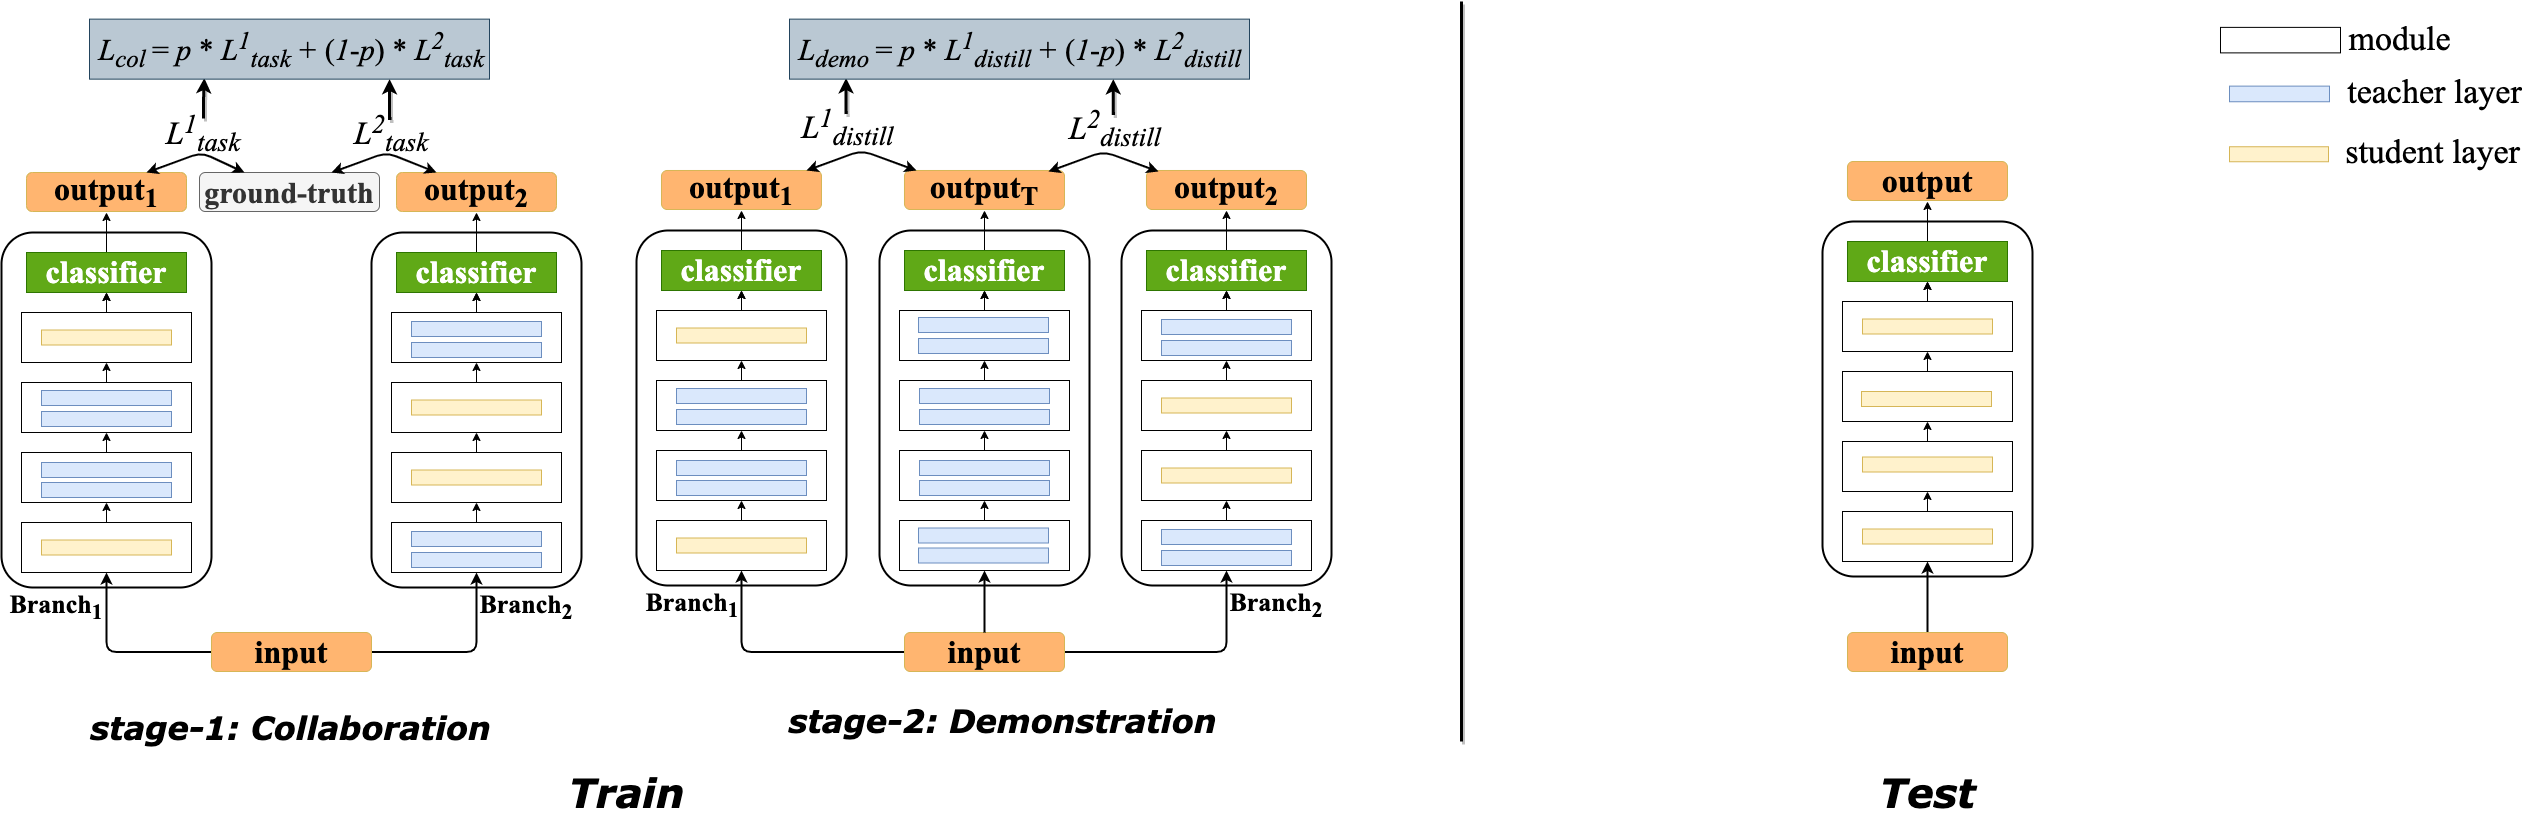
\includegraphics[width=2.0\columnwidth]{figures/overview_1.png}}
    \scalebox{0.88}{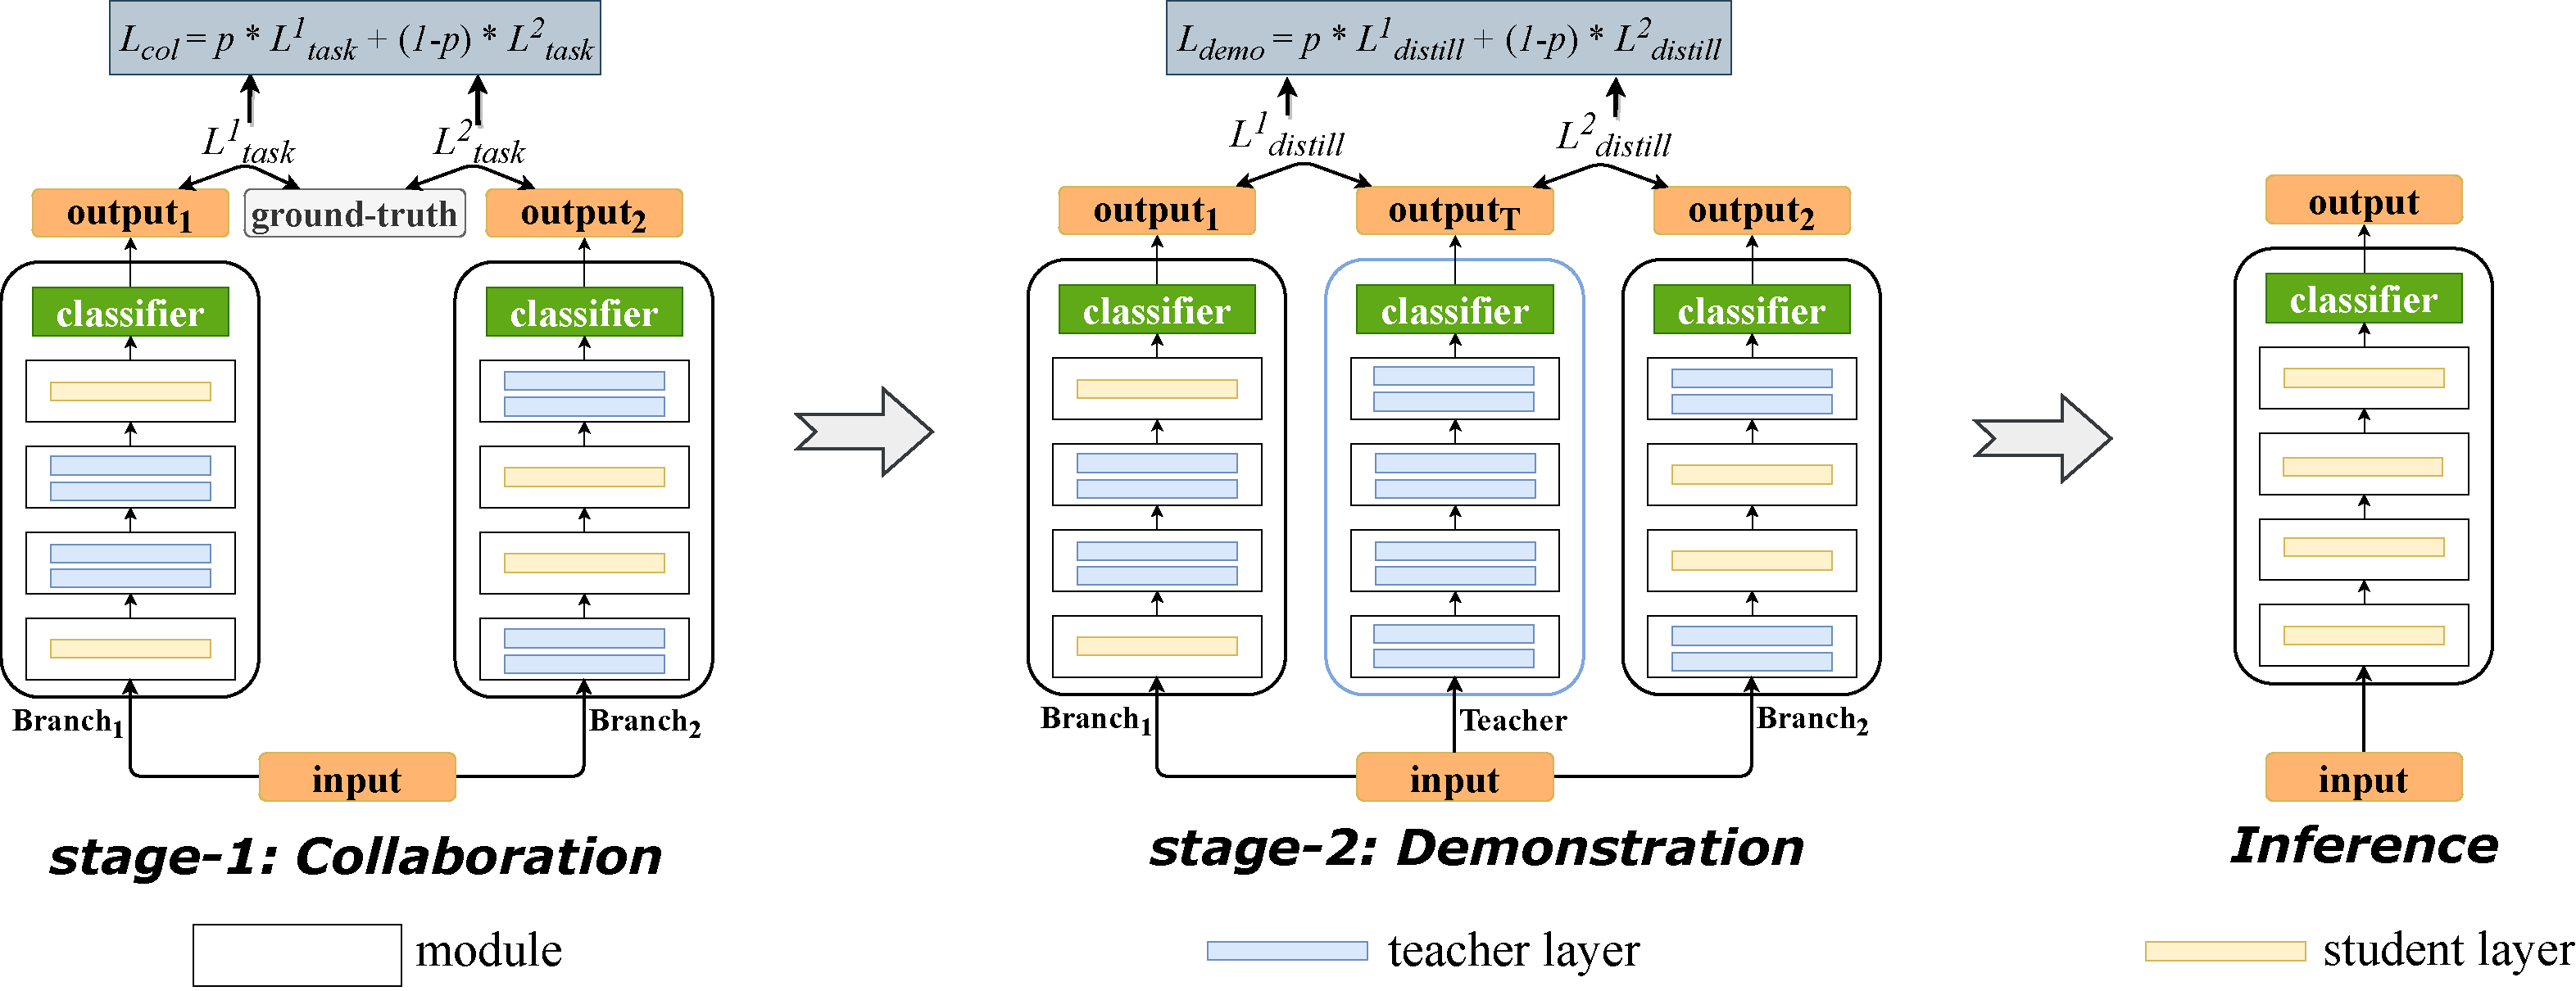
\includegraphics[width=2.0\columnwidth]{figures/lcd.pdf}}
    \caption{An illustrative diagram of LCD based on a novel two-branch container. In this example, we compress an 8-layer teacher into a 4-layer student with a compression ratio $r=2$. During training, each of the two modules at the same depth
    contains either one layer from the student network or $r$ layers from the teacher network controlled by probability $p$. In stage-1, both branches are optimized towards a task-specific objective with ground-truth. In stage-2, both branches are optimized towards a comprehensive knowledge distillation objective with demonstration from the complete teacher network. During testing, all student layers are grouped together as the complete student network.} 
    \label{fig:overview}
\end{figure*}

Our framework LCD holds several merits. Compared to KD-free methods, LCD exploits richer information from both ground-truth and the complete teacher network, making it less likely to overfit small data. Compared to KD-based methods, LCD does not require 
laborious tuning to balance the relative weight between task-specific and distillation objectives. It also avoids potential gradient conflict which is harmful to convergence~\cite{gaml}. Moreover, 
due to the label-free nature in the second stage of LCD, we can easily extend it to a semi-supervised setup by cheap data augmentation such as synonym replacement and paraphrasing to gain further improvement under the same compression ratio.


We conduct experiments on compressing a 12-layer BERT into compact 4/6-layer counterparts for five natural language understanding tasks. Experiment results show that LCD outperforms both KD-based and KD-free methods by significant margins, especially under large 
compression ratio regimes. We perform an ablation study to demonstrate the impact of different technical designs in LCD as well as analyses on both layer and model level that show a better alignment 
between teacher and model compressed by our LCD.

Our contributions are four-fold: (1) We propose a novel two-branch container in which teacher and student layers are interleaved stochastically during training.
(2) We design a two-stage learning framework LCD which enables the student to learn from the teacher in an implicit-to-explicit fashion, essentially combining the advantages of KD-based and KD-free methods.
(3) LCD can easily benefit from cheap data augmentation without human annotation for task-specific labels.
(4) Under the same compression ratio, the model compressed by LCD shows consistent improvements over state-of-the-art baselines on multiple downstream tasks.
